\title{Siftables Emulator: Deployment and Usage}
\author{Singularity Software}
\date{\today}

\documentclass[12pt]{article}
\usepackage[a4paper]{geometry}
\usepackage{makeidx}
\usepackage{lscape}
\usepackage{amsmath}
\usepackage{graphicx}
\usepackage[final]{pdfpages}

\geometry{top=1.0in, bottom=1.0in, left=1.0in, right=1.0in} % Sets the margins

\setlength{\parindent}{0pt} % Fixes the paragraph spacing problem

\renewcommand*\arraystretch{1.5}

\begin{document}

\begin{center}
	\LARGE{Siftables Emulator} \\
	\LARGE{\textit{Deployment and Usage}}\\
	\Large{\textit{Singularity Software}} \\
	\vspace{.05in}
	\normalsize{\today} \\
\end{center}

\section{Install the emulator}
Siftables Emulator is a cross-platform Silverlight application. To install it for the first time:
\begin{enumerate}
\item Build the project using the Release configuration in Visual Studio.
\begin{center}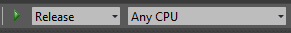
\includegraphics[width=4in]{0-1ReleaseBuild}\end{center}
\item Open [project root]/Siftables/Bin/Release/SiftablesEmulator.html in a Silverlight-compatible web browser.
\begin{center}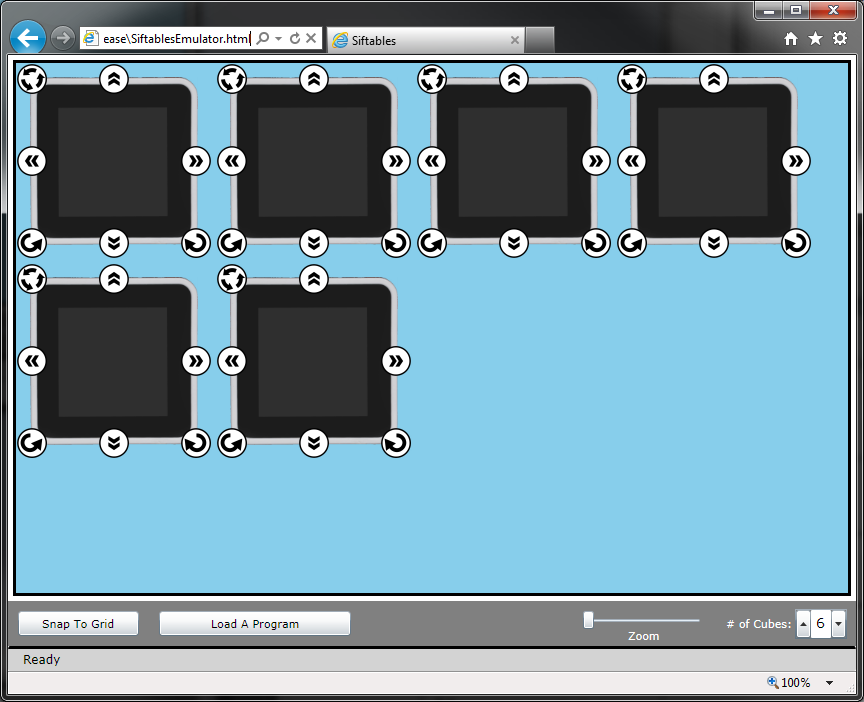
\includegraphics[width=4in]{0-2WebBrowser}\end{center}
\item When the app loads, right click anywhere and choose ``Install Siftables Emulator onto this computer..."
\begin{center}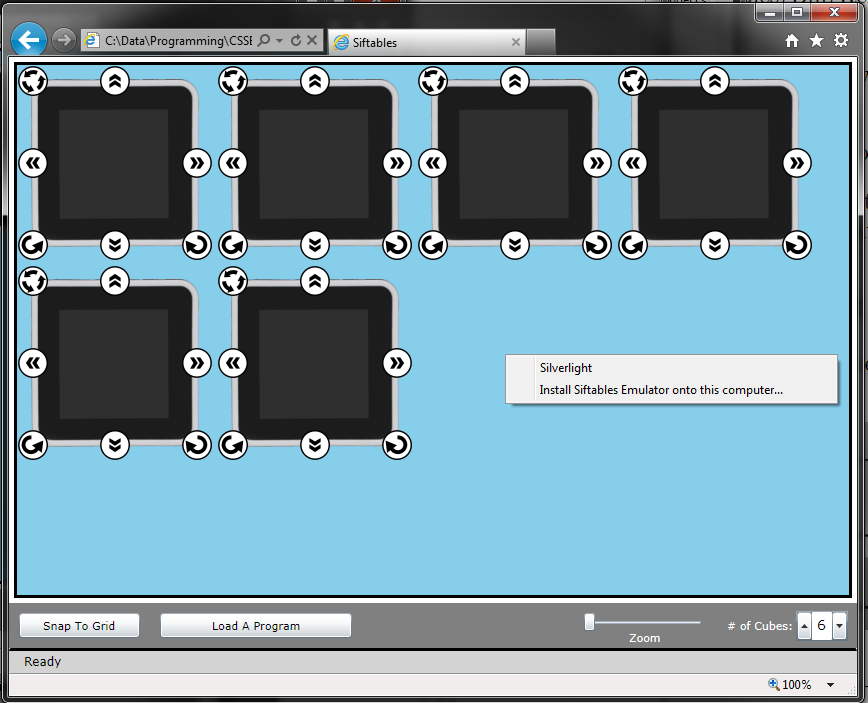
\includegraphics[width=4in]{0-3Install}\end{center}
\item Follow the install wizard, choosing your preferred shortcut locations.
\begin{center}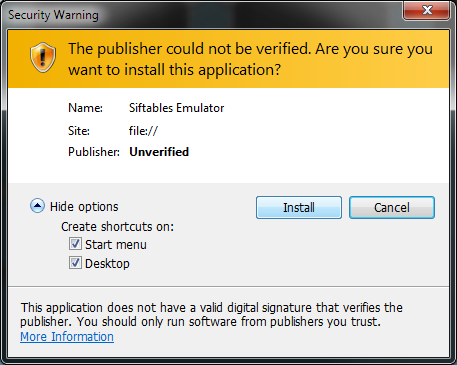
\includegraphics[width=4in]{0-4Install2}\end{center}
\item Siftables Emulator should launch automatically. If not, it can be launched from wherever you opted to install shortcuts in the previous step.
\begin{center}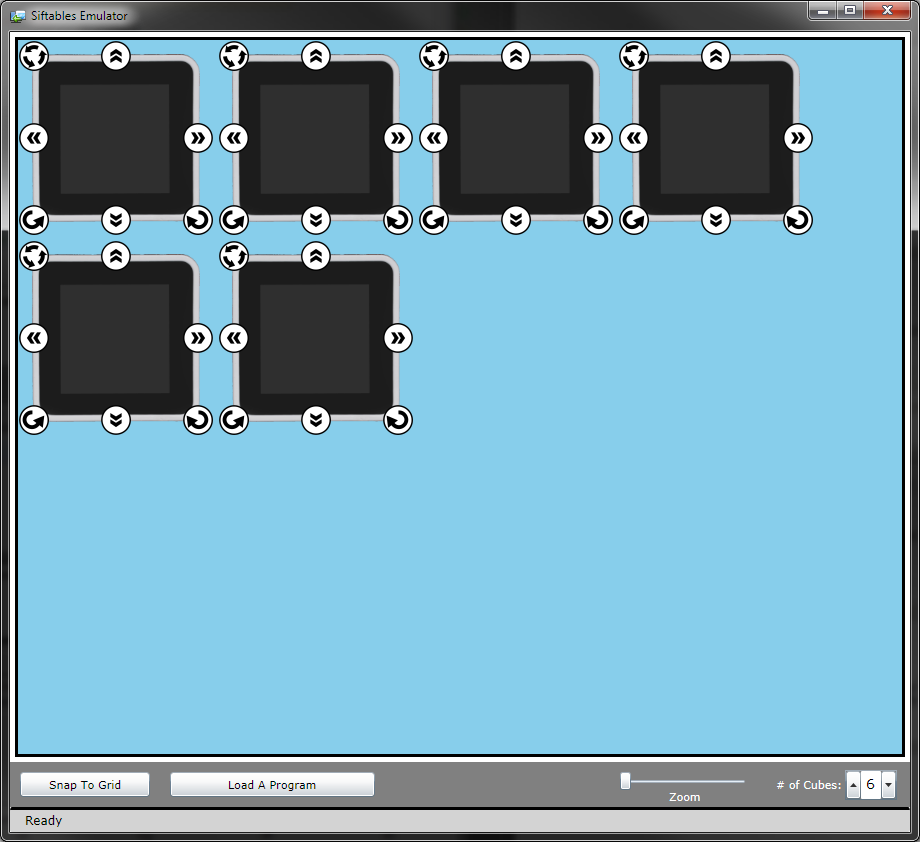
\includegraphics[width=4in]{0-5Installed}\end{center}
\end{enumerate}

\section{Walkthrough: Interact with the emulator}
Once you've launched the emulator, play around! If you get stuck, consult the following mapping of actions on the physical Sifteo Cubes to their digital equivalents.

\begin{center}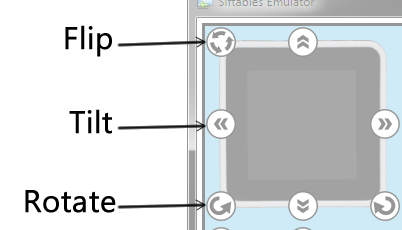
\includegraphics[width=2.5in]{interact}\end{center}
\begin{center}
	\begin{tabular}{ | p{1.5in} | p{4.5in} | }
	\hline
	\textbf{If you want to...}   \\\hline
	Flip the cube,  & click the flip button. \\\hline
	Tilt the cube, & click the tilt button for the direction to tilt [left, up, right, down]. \\\hline
	Rotate the cube, & click the rotate button for the direction to rotate [counterclockwise, clockwise]. \\\hline
	Shake the cube, & drag the cube horizontally back and forth rapidly. \\\hline
	Press the cube, & click the virtual screen. \\\hline
	\end{tabular}\\

	\begin{tabular}{ | p{1.5in} | p{4.5in} | }
	\hline
	\textbf{If you click...}   \\\hline
	Snap to Grid, & the emulator rearranges the cubes into a 4-cube wide grid based on order of cube creation. \\\hline
	Load a Program, & the emulator opens the Load dialog for running a Siftables application DLL. \\\hline
	Zoom,  & the emulator zooms the canvas in (right) or out (left) to a maximum of 2x zoom. \\\hline
	\# of Cubes, & the emulator changes the number of cubes available on the emulator ``screen" to a [maximum of 9, minimum of 1] cubes. \\\hline
	\end{tabular}

\end{center}

\section{Program for the emulator}
\subsection{Application Programming Interface}
Siftables Emulator can be programmed using the official Sifteo API available at\\ http://developer.sifteo.com/. The team believes that our implementation of the API outlined there is complete and is functionally on par with the native Sifteo.dll provided for use with the physical Sifteo cubes. This implementation is a combination of work done by the team specifically for Silverlight and the Siftables project and work done by the Sifteo team. The latter part comes in the form of SifteoExtensions.dll, a partial version of Sifteo.dll decompiled and retargeted to Silverlight with Sifteo's permission.

\subsection{Target the emulator with an existing application}
To target an existing application targeted for Sifteo Cubes to run in Siftables Emulator, follow the instructions in step 1 of the following walkthrough. When you've created the new project, add your existing application files to it.

\subsection{Walkthrough: Prepare and run a new application}
\begin{enumerate}

\item Create a new project for the application.
\begin{enumerate}
\item Select the Silverlight template group in the left pane, then select Silverlight Application in the center.
\item Give the application a name and a location. We recommend not creating a directory for the solution.
\begin{center}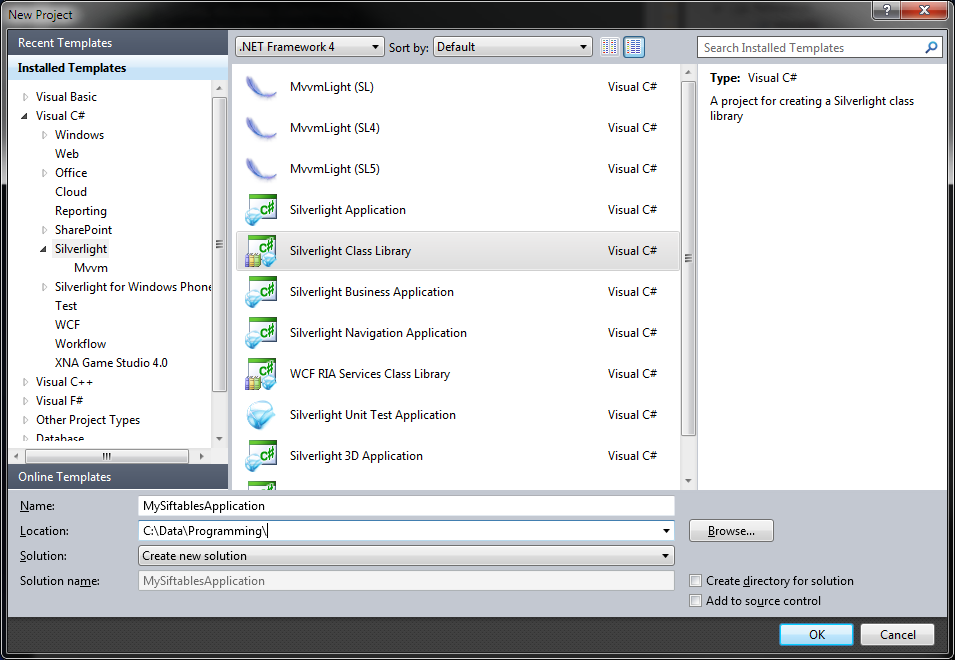
\includegraphics[width=4in]{1-1-NewProjectDialog}\end{center}
\item Ensure that you use Silverlight version 5.
\begin{center}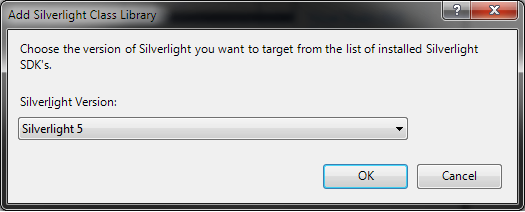
\includegraphics[width=4in]{1-2-NewSilverlightApp}\end{center}
\item Add Sifteo.dll and SifteoExtensions.dll to the project references. Note that those DLLs will only exist if you have already built the Release configuration of the emulator as specified in the installation instructions.
\begin{center}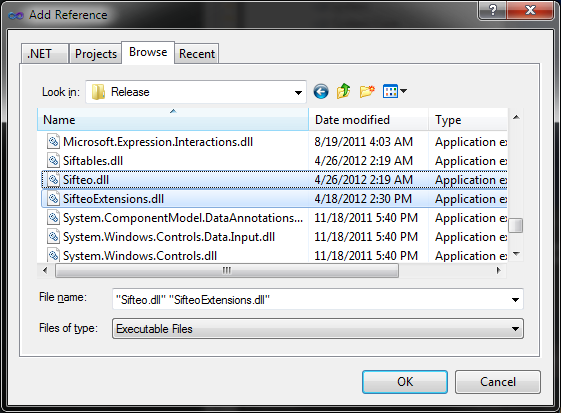
\includegraphics[width=4in]{1-3-AddReferences}\end{center}
\end{enumerate}

\item Build a blank runnable application.
\begin{enumerate}
\item Create a new class.
\item Have it extend BaseApp.
\begin{center}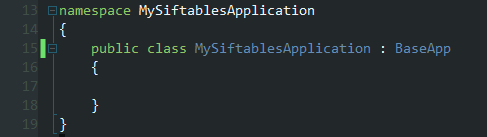
\includegraphics[width=4in]{2-1BlankApp}\end{center}
\item Have it use the Sifteo namespace (Visual Studio should offer to do this for you).
\item Build the solution. Note the location of the DLL in Output.
\begin{center}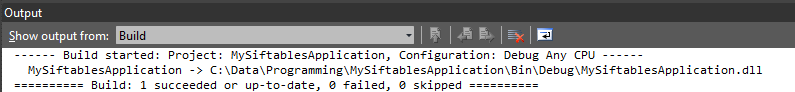
\includegraphics[width=4in]{2-2Output}\end{center}
\end{enumerate}

\item Run the blank application in the emulator.
\begin{enumerate}
\item Launch the emulator.
\item Click ``Load A Program".
\item Select the DLL built in the previous step.
\item Click Open.
\begin{center}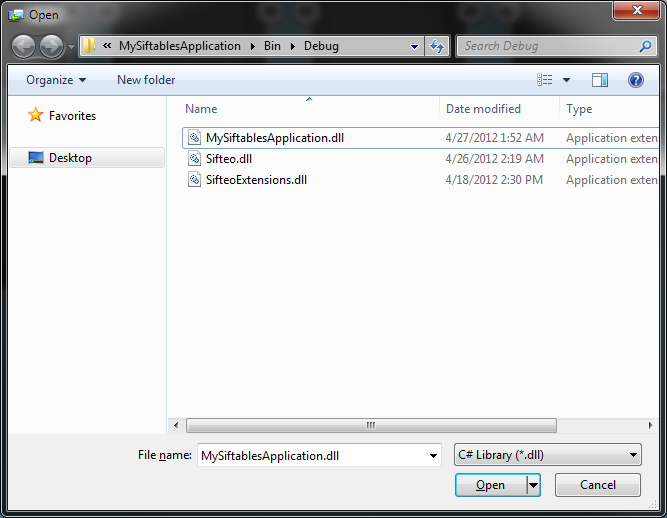
\includegraphics[width=4in]{3-1Open}\end{center}
\end{enumerate}
At this point, you have a fully runnable Siftables application. It doesn't do anything... but that part is up to you!\\

\end{enumerate}

\subsection{Example: Respond to cube events}
All cube interactions appear to your program as events. If you want to do something when one of those interactions occurs, simply add a handler to the appropriate event.

	\begin{tabular}{ | p{2in} | p{4in} | }
	\hline
	\textbf{If you want to respond when the user...} &  \\\hline
	Flips the cube,  & bind to cube.NotifyCubeFlip. \\\hline
	Tilts the cube, & bind to cube.NotifyCubeTilt. \\\hline
	Rotates the cube, & you can't - at least, you can't directly. The orientation of the cube only affects operations that use neighboring to make multiple cubes interact. \\\hline
	Shakes the cube, & bind to cube.NotifyShakeStarted and/or cube.NotifyShakeStopped. \\\hline
	Presses the cube, & bind to cube.NotifyButtonPressed. \\\hline
	Has neighbored cubes, & access cube.Neighbors. \\\hline
	\end{tabular}\\
	
\subsection{Example applications}
Example applications are located in [project root]/Applications.

\begin{itemize}
\item CubeTestApp has examples of how to respond to most cube interactions and is a good place to start.
\item ChangingColorsApp is an example of how to work with neighbored cubes.
\item FractionOrderingApp uses neighboring and images in a simple ordering game.
\end{itemize}

\end{document}
